\documentclass[12pt]{article}

\usepackage[margin=1in]{geometry}
\usepackage{graphicx}
\usepackage{float}
\usepackage{amsmath, amssymb, amsthm, dsfont}
\usepackage{setspace}
\usepackage{parskip}
\usepackage{hyperref}
\usepackage{tabularx}
\usepackage{booktabs}
\usepackage[labelsep=period]{caption}

\title{STAT 236 Final Project}
\author{Amrit Chadha, Faris Doughan}
\date{October 2026}

\newtheorem{theorem}{Theorem}
\newtheorem{lemma}{Lemma}
\newtheorem{proposition}{Proposition}
\newtheorem{conjecture}{Conjecture}

\begin{document}

\begin{titlepage}
    \centering
    \vspace*{0.24\textheight}
    {\Huge \textbf{STAT 236 Final Project}}\\[1.5em]
    {\Large Sparse Submatrix Detection}\\[3em]
    {\large Amrit Chadha, Faris Doughan}\\[1em]
    {\large Fall 2026}
\end{titlepage}

\section{Introduction}

Sparse submatrix detection is a problem in high-dimensional statistics concerned with detecting a small, structured signal hidden within a large noisy matrix. As with many of the topics covered in this course, a central question is how the size of the planted submatrix and the strength of its signal affect our ability to distinguish it from random noise.


An important feature of this problem is the distinction between statistical and computational limits of detection. From a purely statistical perspective, we would like to determine the weakest signal for which any hypothesis test can reliably distinguish the two cases, regardless of its computational cost. However, a statistically optimal procedure may require searching over an enormous number of possible submatrices. We therefore also ask how strong the signal must be for detection to be possible using an efficient algorithm, such as one running in polynomial time.

The problem was studied by Butucea and Ingster (2013) \cite{BI2013}, who established asymptotic detection boundaries for the Gaussian model, and later by Ma and Wu (2015) \cite{MW2015}, who investigated the computational limitations of detection. Our hope is to develop the theory in an accessible way, so that an undergraduate or graduate student can follow the main arguments and gain an understanding of the basic literature. To this end, we primarily consider square matrices with square planted submatrices and a common positive mean shift.

The papers contain substantial technical detail, and working through every argument in full generality would be beyond what we could reasonably understand within the scope of this project. We explain the main detection guarantees in the text and put the calculations in the appendix. We then compare the detection regimes and discuss the stronger requirements for recovering the affected rows and columns.

Table~\ref{tab:methods} summarizes the procedures discussed in this report.
Here, $n$ is the number of rows and columns in the observed matrix,
$k$ is the number of affected rows and columns, and $\mu$ is their
common mean shift. The noise entries are independent standard Gaussian
variables. We assume $k\to\infty$ and $k=o(n)$. For comparisons with
polynomial block growth, we write $k=\lfloor n^\gamma\rfloor$, where
$0<\gamma<1$.

\clearpage



\begin{table}[!ht]
\centering
\small
\setlength{\tabcolsep}{3.5pt}
\renewcommand{\arraystretch}{1.2}
\caption{Detection and recovery procedures}
\label{tab:methods}
\begin{tabularx}{\textwidth}{@{}>{\raggedright\arraybackslash}p{2.3cm}
  >{\raggedright\arraybackslash}p{2.5cm}
  >{\raggedright\arraybackslash}p{1.8cm}
  >{\raggedright\arraybackslash}X
  >{\raggedright\arraybackslash}p{2.1cm}@{}}
\toprule
\textbf{Procedure} & \textbf{Paper} & \textbf{Goal}
& \textbf{Regime and guarantee} & \textbf{Cost} \\
\midrule
Sum & Butucea and Ingster~\cite{BI2013} & Detection
& Statistically rate optimal for $\gamma>2/3$. Reliable when
$\mu k^2/n\to\infty$.
& $O(n^2)$ \\
\addlinespace
Scan & Butucea and Ingster~\cite{BI2013} & Detection
& Attains the statistical exponent boundary for $\gamma<2/3$.
The sufficient signal condition is given in Section~\ref{sec:scan}.
& Exhaustive search \\
\addlinespace
Maximum entry & Ma and Wu~\cite{MW2015} & Detection
& A sufficient regime is
$\liminf\mu/(2\sqrt{\log n})>1$, where individual entries carry
strong signals.
& $O(n^2)$ \\
\addlinespace
Sum and scan & Butucea and Ingster~\cite{BI2013} & Detection
& Combines the two detection regimes and attains the statistical
boundary.
& Includes exhaustive scan \\
\addlinespace
Maximizing block sum & Butucea, Ingster and Suslina~\cite{BIS2015}
& Recovery
& Attains the sharp statistical boundary for exact recovery stated
in Section~\ref{sec:exact-recovery}.
& Exhaustive search \\
\addlinespace
Spectral projection & Cai, Liang and Rakhlin~\cite{CLR2017}
& Recovery
& For $k/\sqrt n\to\infty$. Succeeds when
$\mu\geq C(\sqrt n/k+\sqrt{\log n/k})$.
& Polynomial time \\
\addlinespace
Thresholded spectral projection & Cai, Liang and Rakhlin~\cite{CLR2017}
& Recovery
& For $k/\sqrt n\to0$. Succeeds when
$\mu/\sqrt{\log(n/k^2)}\to\infty$.
& Polynomial time \\
\bottomrule
\end{tabularx}

\medskip
\begin{minipage}{\textwidth}
\footnotesize
The max and spectral rows give sufficient conditions. Here, $C$ is a
sufficiently large absolute constant. The exponent comparisons use
strict inequalities, as explained in Section~\ref{sec:comparison}.
\end{minipage}
\end{table}

\clearpage

\section{Detection}\label{sec:detection}

\subsection{The Model and Testing Error}

We begin with the standard Gaussian formulation of the problem. We observe
a matrix $X\in\mathbb R^{n\times n}$ and consider the null hypothesis
\[
H_0\quad X_{ij}\overset{\mathrm{iid}}{\sim}N(0,1)
\]
against the alternative
\[
H_1\quad X_{ij}\overset{\mathrm{ind}}{\sim}
N\left(\mu\mathds{1}_{\{i\in S,\,j\in T\}},1\right)
\]
where $[n]=\{1,\ldots,n\}$ and $S,T\subseteq[n]$ are unknown subsets
with $|S|=|T|=k$. The signal strength is $\mu>0$, and $\mathds{1}$
denotes the indicator function. Thus, under the alternative, there is an unknown $k\times k$
submatrix whose entries have mean $\mu$, while all other entries have
mean zero. The entries are independent under both hypotheses, and the
affected rows and columns need not be consecutive.

Our goal is to understand how the difficulty of detection changes as the
matrix becomes larger. As $n$ increases, the block size and signal
strength may also change, so we write $k=k_n$ and $\mu=\mu_n$. For
instance, a larger block may allow us to detect a weaker signal because
more affected entries contribute evidence for the alternative. We seek
conditions on $n$, $k$, and $\mu$ under which the testing errors tend to
zero. Throughout the asymptotic results, we assume $k\to\infty$ and
$k=o(n)$.

Write $P_0$ for the null distribution and $P_{S,T,\mu}$ for the
distribution under an alternative with affected rows $S$ and columns
$T$. A test $\varphi_n$ takes value one when we reject $H_0$ and zero
otherwise. We allow the test to depend on $n$, since its input and
rejection threshold may change with the matrix size. Its total testing
error is
\[
R_n(\varphi_n)
=P_0(\varphi_n=1)
+\sup_{\substack{S,T\subseteq[n]\\|S|=|T|=k}}
P_{S,T,\mu}(\varphi_n=0)
\]
The first term is the false positive rate. The second is the largest
probability of missing a signal over all possible block locations. We
say that reliable detection is achieved if $R_n(\varphi_n)\to0$, so that
both errors vanish. This is the minimax testing criterion used by
Butucea and Ingster~\cite{BI2013} and Ma and Wu~\cite{MW2015}, written
in our notation.

\subsection{The Sum Test}

The first, and most natural (in fact, we both had thought of this before
even looking at any papers), approach is to sum all entries in the
matrix and compare the result with what is expected under $H_0$. As
only detection is required, such a method is able to aggregate the
effects of individually small mean shifts without identifying the
specific indices. We define
\[
T_{\mathrm{sum}}=\frac1n\sum_{i=1}^n\sum_{j=1}^n X_{ij}
\]
This statistic is $N(0,1)$ under $H_0$ and $N(\Delta_n,1)$ under any
alternative. Here, $\Delta_n=\mu k^2/n$ is the mean shift of the
normalized sum. We reject when $T_{\mathrm{sum}}>c_n$, where $c_n$
is the rejection threshold. Theorem 2.1 of Butucea and
Ingster~\cite{BI2013} shows that reliable detection is possible when
$\Delta_n\to\infty$. We can then choose $c_n$ to tend to infinity
while staying below a fixed fraction of $\Delta_n$. Their error calculation is
given in Appendix~\ref{app:sum}.

Computing the sum takes $O(n^2)$ operations, which is linear in the
number of observed entries, and only $O(1)$ additional storage if the
entries are processed sequentially. Its limitation is statistical in the sense that the
unnormalized sum collects a mean shift of $\mu k^2$, but also noise
with standard deviation $n$. For sufficiently small blocks, the many
unaffected entries can obscure the signal. This motivates procedures
that concentrate evidence within candidate submatrices instead.

\subsection{The Scan Test}\label{sec:scan}

A natural alternative is to sum only over a candidate submatrix. Since
the affected rows and columns are unknown, we consider all possible
candidates and reject if any candidate has a sufficiently large sum.
For each candidate with row set $A$ and column set $B$, both of size
$k$, let $Z_{A,B}=k^{-1}\sum_{i\in A,j\in B}X_{ij}$ be its
normalized sum. There are $M_n=\binom nk^2$ candidates. The scan
statistic is the largest of their normalized sums
\[
T_{\mathrm{scan}}
=\max_{\substack{A,B\subseteq[n]\\|A|=|B|=k}}Z_{A,B}
\]
Each candidate sum is standard
normal under $H_0$, while the true block satisfies
$Z_{S,T}\sim N(\mu k,1)$ under $H_1$. However, searching over many
candidates makes it more likely that some sum will be large purely
because of noise. The threshold must account for this search.

Let $h_n$ denote the rejection threshold, so that we reject $H_0$ when
$T_{\mathrm{scan}}>h_n$. Butucea and Ingster~\cite[Theorem 2.1]{BI2013}
choose $h_n=\sqrt{2\log M_n}$. This threshold grows with the number
of candidates to control false positives from the search. With this
choice, they show that reliable detection is possible when
\[
\liminf_{n\to\infty}\frac{\mu^2k}{4\log(n/k)}>1
\]
Thus, it is sufficient for the entrywise mean shift $\mu$ to exceed
$2\sqrt{\log(n/k)/k}$ by a fixed factor. Appendix~\ref{app:scan} follows
their proof, including the control of the maximum over dependent
candidate sums.

The difficulty is computational. The scan requires knowledge of $k$,
and exhaustive enumeration examines $M_n$ candidates. Computing each
sum separately takes $O(k^2M_n)$ operations, which is superpolynomial
under our assumptions on $k$. A better statistical guarantee can
therefore come at a substantial computational cost.

\subsection{The Maximum-Entry Test}

Another natural approach is related to the sparse inference problems
discussed in the course, where we considered minimum-$p$ tests and
Tukey's higher criticism. A minimum-$p$ test looks for a single
unusually significant observation, while higher criticism can collect
evidence from an excess of small $p$-values. In our setting, the first
approach corresponds to testing whether any matrix entry is unusually
large. Accordingly, define
\[
T_{\mathrm{max}}=\max_{1\leq i,j\leq n}X_{ij}
\]
Let $\Phi$ denote the standard normal distribution function. Since the
one-sided $p$-value for each entry is $p_{ij}=1-\Phi(X_{ij})$, we have
$\min_{i,j}p_{ij}=1-\Phi(T_{\mathrm{max}})$. Thus, this is precisely a
minimum-$p$ test.

For this test, let $u_n$ denote the rejection threshold, so that we
reject when $T_{\mathrm{max}}>u_n$. Ma and Wu~\cite[Lemma 1]{MW2015}
choose $u_n=\sqrt{(4+\varepsilon)\log n}$, where $\varepsilon>0$
is a fixed constant. Their
Theorem 2, condition (17), gives the sufficient regime
\[
\liminf_{n\to\infty}\frac{\mu}{2\sqrt{\log n}}>1
\]
Taking $\varepsilon$ sufficiently small then makes the total error tend
to zero. The bound they use is stated and explained in
Appendix~\ref{app:max}.

Like the sum, the maximum can be computed in $O(n^2)$ operations with
$O(1)$ additional storage. It requires neither the block size nor its
location. However, it does not exploit the shared row and column
structure, since permuting all matrix entries leaves the statistic unchanged.

\section{Comparison}\label{sec:comparison}

\subsection{Statistical Detection Regimes}

The sum and scan tests differ in how they use the affected entries.
The sum gains from having many small shifts across the matrix. The
scan avoids much of the noise from unaffected entries, but must
compensate for the number of possible block locations. Butucea and
Ingster~\cite[Theorem 2.1]{BI2013} combine the two tests, rejecting
whenever either rejects, so that the combined procedure succeeds under
either of the conditions above.

Their lower bound shows why both conditions matter. Write
$R_n^\star=\inf_\varphi R_n(\varphi)$, where the infimum is over all
tests based on the full matrix. In the square case, their Theorem 2.2
gives
\[
\frac{\mu k^2}{n}\longrightarrow0
\qquad\text{and}\qquad
\limsup_{n\to\infty}\frac{\mu^2k}{4\log(n/k)}<1
\quad\Longrightarrow\quad R_n^\star\longrightarrow1
\]
The additional balance assumptions in the theorem hold in this square
setting, and its proof uses alternatives with a common mean shift
\cite[Section 5.1]{BI2013}. Thus, when both ways of accumulating
signal are too weak, no other test can make the errors vanish. The
strict inequalities do not settle all critical sequences at equality.

To see which test is useful for different block sizes, follow Ma and
Wu~\cite[Section 1.2]{MW2015} and write
$k=\lfloor n^\gamma\rfloor$ and $\mu=n^{-\beta}$, with
$0<\gamma<1$ and $0<\beta<1$. Larger $\beta$ means a weaker signal.
Their statistical boundary, in our notation, is
\[
\beta_{\mathrm{stat}}
=\max\left\{\frac\gamma2,\,2\gamma-1\right\}
\]
Detection is statistically possible for
$\beta<\beta_{\mathrm{stat}}$ and impossible for
$\beta>\beta_{\mathrm{stat}}$.

For $2/3<\gamma<1$, which Ma and Wu call the moderately sparse regime,
the sum attains the statistical rate. The block contributes enough
total signal that searching for its location does not improve this
rate. For $0<\gamma<2/3$, their highly sparse regime, scanning attains
the statistical boundary at weaker signals than the sum. At
$\gamma=2/3$, the two exponent expressions agree. The original
conditions must still be used to account for logarithmic factors.

The max guarantee requires individual mean shifts larger than
$2\sqrt{\log n}$ by a fixed factor. These signals are stronger than those described by
$\mu=n^{-\beta}$. The max is inexpensive and useful when individual
entries are informative, but Ma and Wu's stated sufficient bound does
not give a sharp classification of its power for every block size.

\subsection{Computation}

Both the sum and max take time linear in the number of entries. The
statistically stronger scan guarantee for small blocks is obtained by
a search whose direct implementation is superpolynomial. This alone
does not prove that efficient detection is impossible, since another
algorithm might avoid the search.

Ma and Wu~\cite[Theorem 2 and Figure 1]{MW2015} address this question
under the planted-clique hypothesis. This hypothesis rules out reliable
randomized polynomial-time detection of a planted clique of size
$N^\rho$, for fixed $0<\rho<1/2$, in a graph drawn from $G(N,1/2)$.
Their reduction shows that an efficient submatrix detector in certain
regimes would also give an efficient detector for such a clique.

Ma and Wu allow a
rectangular affected block with at least $k$ rows and columns and means
bounded below by $\mu$. They formulate the computational theorem for
a discretized Gaussian model that is statistically equivalent to the
continuous model asymptotically. Their impossibility statement is for
that larger alternative class. It does not automatically become an
impossibility theorem for our exact-size, common-mean alternative.

For their model, the computational exponent boundary is
$\beta_{\mathrm{comp}}=\max\{0,2\gamma-1\}$. When
$0<\gamma<2/3$, the interval
$\beta_{\mathrm{comp}}<\beta<\beta_{\mathrm{stat}}$ is statistically
possible but computationally intractable under that hypothesis. When
$2/3<\gamma<1$, the two boundaries coincide and the sum already
achieves the statistical rate. These are strict exponent comparisons.
Logarithmic factors can matter at the boundaries.

These asymptotic results do not determine the finite-sample power
ordering of the tests. Our
simulations will compare power at a common significance level and
record the computational cost. Any heuristic approximation to the scan
will be distinguished from the exhaustive statistic. Butucea and
Ingster also use a heuristic search in their numerical study
\cite[Section 3]{BI2013}.

\section{Recovery}\label{sec:recovery}

Detection establishes that an affected group exists, but does not tell
us which rows and columns belong to it. Recovering these indices may
be necessary if we want to investigate the group further. A recovery
procedure returns estimates $\widehat S$ of the affected rows and
$\widehat T$ of the affected columns. We require
\[
\sup_{\substack{S,T\subseteq[n]\\|S|=|T|=k}}
P_{S,T,\mu}\bigl((\widehat S,\widehat T)\ne(S,T)\bigr)
\longrightarrow0
\]
This is exact recovery. Both index sets must be entirely correct, so
even one incorrect row or column counts as an error.

\subsection{Exact Recovery by Scanning}\label{sec:exact-recovery}

Butucea, Ingster and Suslina~\cite{BIS2015} study this problem using
the estimator
\[
(\widehat S,\widehat T)
=\underset{\substack{A,B\subseteq[n]\\|A|=|B|=k}}{\arg\max}
\sum_{i\in A,j\in B}X_{ij}
\]
This is the same search used by the scan test, but now we retain the
maximizing indices. The true block must now have a larger sum than every incorrect
candidate, including candidates that differ by just one row or column.

For $k\to\infty$ and $k=o(n)$, their Theorems 2.1 and 2.3 give the
sharp square-block recovery boundary
\[
\mu_{\mathrm{rec}}^\star
\sim\max\left\{
\frac{\sqrt{2\log k}+\sqrt{2\log(n-k)}}{\sqrt k},\,
2\sqrt{\frac{\log(n/k)}{k}}
\right\}
\]
A fixed multiplicative separation above this boundary permits exact
recovery, while a fixed separation below it makes the minimax
probability of an incorrect recovery tend to one.

The first term explains a difficulty that detection does not have.
Even if the true columns were known, the affected rows would have to
be separated from every unaffected row. The standardized row sums
have mean shift $\mu\sqrt k$, which must overcome both unusually
large noise rows and unusually small affected rows. The second term
accounts for the many competing block locations. 

The exhaustive estimator has the same computational difficulty as
the scan test. We next consider an efficient alternative.

\subsection{Spectral Recovery}

Cai, Liang and Rakhlin~\cite{CLR2017} approach recovery using the
singular vectors of the observed matrix. The mean matrix is
$M=\mu\mathds{1}_S\mathds{1}_T^\top$, which has rank one. Here, $\mathds{1}_S$ and $\mathds{1}_T$ are the indicator vectors of
the affected rows and columns. The left and right singular vectors of
$M$ are proportional to these vectors.

Their Algorithm 1 computes the leading left singular vector
$\widehat u$ and leading right singular vector $\widehat v$ of $X$. It then forms the column scores
$\widehat u^\top X_{\cdot j}$ and row scores
$X_{i\cdot}\widehat v$. Under their signal condition,
the affected and unaffected indices form two separated groups of
scores, and a threshold between the groups recovers the index sets.

For square blocks with $k/\sqrt n\to\infty$, their Lemma 1 gives a
sufficiently large absolute constant $C$ such that exact recovery
succeeds whenever
\[
\mu\geq C\left(\frac{\sqrt n}{k}
+\sqrt{\frac{\log n}{k}}\right)
\]
The authors suggest iterative power methods for the leading singular
vectors, avoiding the search over block locations.

\subsection{Smaller Blocks and Computational Limits}

For $k/\sqrt n\to0$, Cai, Liang and Rakhlin first reduce the noise by
soft-thresholding each entry. At a threshold level $t>0$, this replaces
an entry $x$ by
$\eta_t(x)=\operatorname{sign}(x)(|x|-t)_+$, where $(a)_+=\max\{a,0\}$.
They then apply the same
spectral projection and clustering steps to the thresholded matrix.
Their Theorem 4 gives exact recovery when
\[
\frac{\mu}{\sqrt{\log(n/k^2)}}\longrightarrow\infty
\]
with a threshold level $t$ of order $\sqrt{\log(n/k^2)}$.

Under a hidden-clique recovery hypothesis, their Theorems 2--4 give a
gap between statistical and computational recovery in the broader
sub-Gaussian model, even in dense regimes where the detection gap
disappears. The spectral upper bounds apply to our Gaussian
observations, while the computational lower bounds are minimax
statements over the paper's larger noise class.

\clearpage
% Automatically generated from results/summary.csv. Do not hand-edit values.
% IMPORTANT: estimates are finite-sample Monte Carlo results, not claims of asymptotic optimality.
\section{Simulations}\label{sec:simulations}
We simulated independent $n\times n$ matrices with $X_{ij}\sim N(0,1)$ under the null
and added a positive mean shift $\mu$ to a uniformly sampled, arbitrarily located
$k\times k$ block under the alternative. The block was unknown to each procedure.
All tests used a one-sided nominal level $\alpha=0.05$, with $1{,}500$
independent null samples per configuration to calibrate their rejection
thresholds; the combined sum-or-scan procedure used a Bonferroni split of
$\alpha/2$ between its two component thresholds. We evaluated each configuration
on $600$ independently generated null matrices and $600$ independently generated
alternatives at each signal strength. The tests used paired matrices within
each replicate. We recorded empirical Type I error and detection power, and
reported Wilson $95\%$ confidence intervals for each conditional binomial
proportion. Calibration variability is not included in those intervals.

For exact recovery, we evaluated $600$ independent alternative matrices per
configuration and recorded success only when \emph{both} affected index sets
were recovered exactly. The exhaustive scan and maximizing-block estimator
were computed exactly by enumerating row subsets and optimizing the column
subset for each. Consequently, exhaustive procedures were evaluated only
on small matrices. We used the leading singular vectors for spectral projection;
thresholded spectral projection applied fixed soft thresholding before
computing those vectors. The mean shift grid and threshold choices were
fixed before evaluating test outcomes. All random draws used the seeded
NumPy generator; the exact code, per-trial records and figures are archived
with the project repository.

\begin{table}[t]
\centering\small
\caption{Selected finite-sample simulation results. Each entry is an estimated detection power or exact-recovery probability and its Wilson $95\%$ interval from $600$ replications.}
\begin{tabular}{@{}llcll@{}}\toprule
Configuration & $(n,k)$ & $\mu$ & Procedure & Estimate (95\% CI) \\
\midrule
D1 & $(16,4)$ & $1.2$ & Global sum & $34.3\%\;[30.6,\,38.2]\%$ \\
D1 & $(16,4)$ & $1.2$ & Exhaustive scan & $63.7\%\;[59.7,\,67.4]\%$ \\
D1 & $(16,4)$ & $1.2$ & Maximum entry & $17.3\%\;[14.5,\,20.6]\%$ \\
D3 & $(64,16)$ & $0.6$ & Global sum & $77.8\%\;[74.3,\,81.0]\%$ \\
D3 & $(64,16)$ & $0.6$ & Column pooling & $36.3\%\;[32.6,\,40.3]\%$ \\
D3 & $(64,16)$ & $0.6$ & Maximum entry & $8.3\%\;[6.4,\,10.8]\%$ \\
D4 & $(64,4)$ & $2.5$ & Global sum & $14.3\%\;[11.8,\,17.4]\%$ \\
D4 & $(64,4)$ & $2.5$ & Maximum entry & $50.3\%\;[46.3,\,54.3]\%$ \\
D4 & $(64,4)$ & $2.5$ & Column pooling & $15.2\%\;[12.5,\,18.3]\%$ \\
R1 & $(16,4)$ & $1.75$ & Exhaustive maximizer & $63.2\%\;[59.2,\,66.9]\%$ \\
R1 & $(16,4)$ & $1.75$ & Spectral projection & $44.8\%\;[40.9,\,48.8]\%$ \\
R4 & $(64,4)$ & $3$ & Spectral projection & $74.2\%\;[70.5,\,77.5]\%$ \\
R4 & $(64,4)$ & $3$ & Thresholded spectral & $90.2\%\;[87.5,\,92.3]\%$ \\
\bottomrule\end{tabular}\label{tab:simulation-results}
\end{table}

Figure~\ref{fig:power-curves} compares detection power, while
Figure~\ref{fig:recovery-curves} shows exact-recovery probabilities.
In the $(n,k)=(16,4)$ setting, scanning improves power over the global sum
at moderate shifts, reflecting its ability to concentrate on a sparse block.
For $(64,16)$, aggregation becomes more effective at weak shifts, whereas
for $(64,4)$ the maximum-entry test can outperform global aggregation when
individual signals are large. Exact recovery can require substantially more
signal than simple detection; in the $(64,4)$ example soft-thresholded
spectral projection improves over the unthresholded spectral baseline at
intermediate shifts. These finite-sample comparisons do not establish
computational lower bounds or prove asymptotic phase transitions.

\begin{figure}[t]\centering
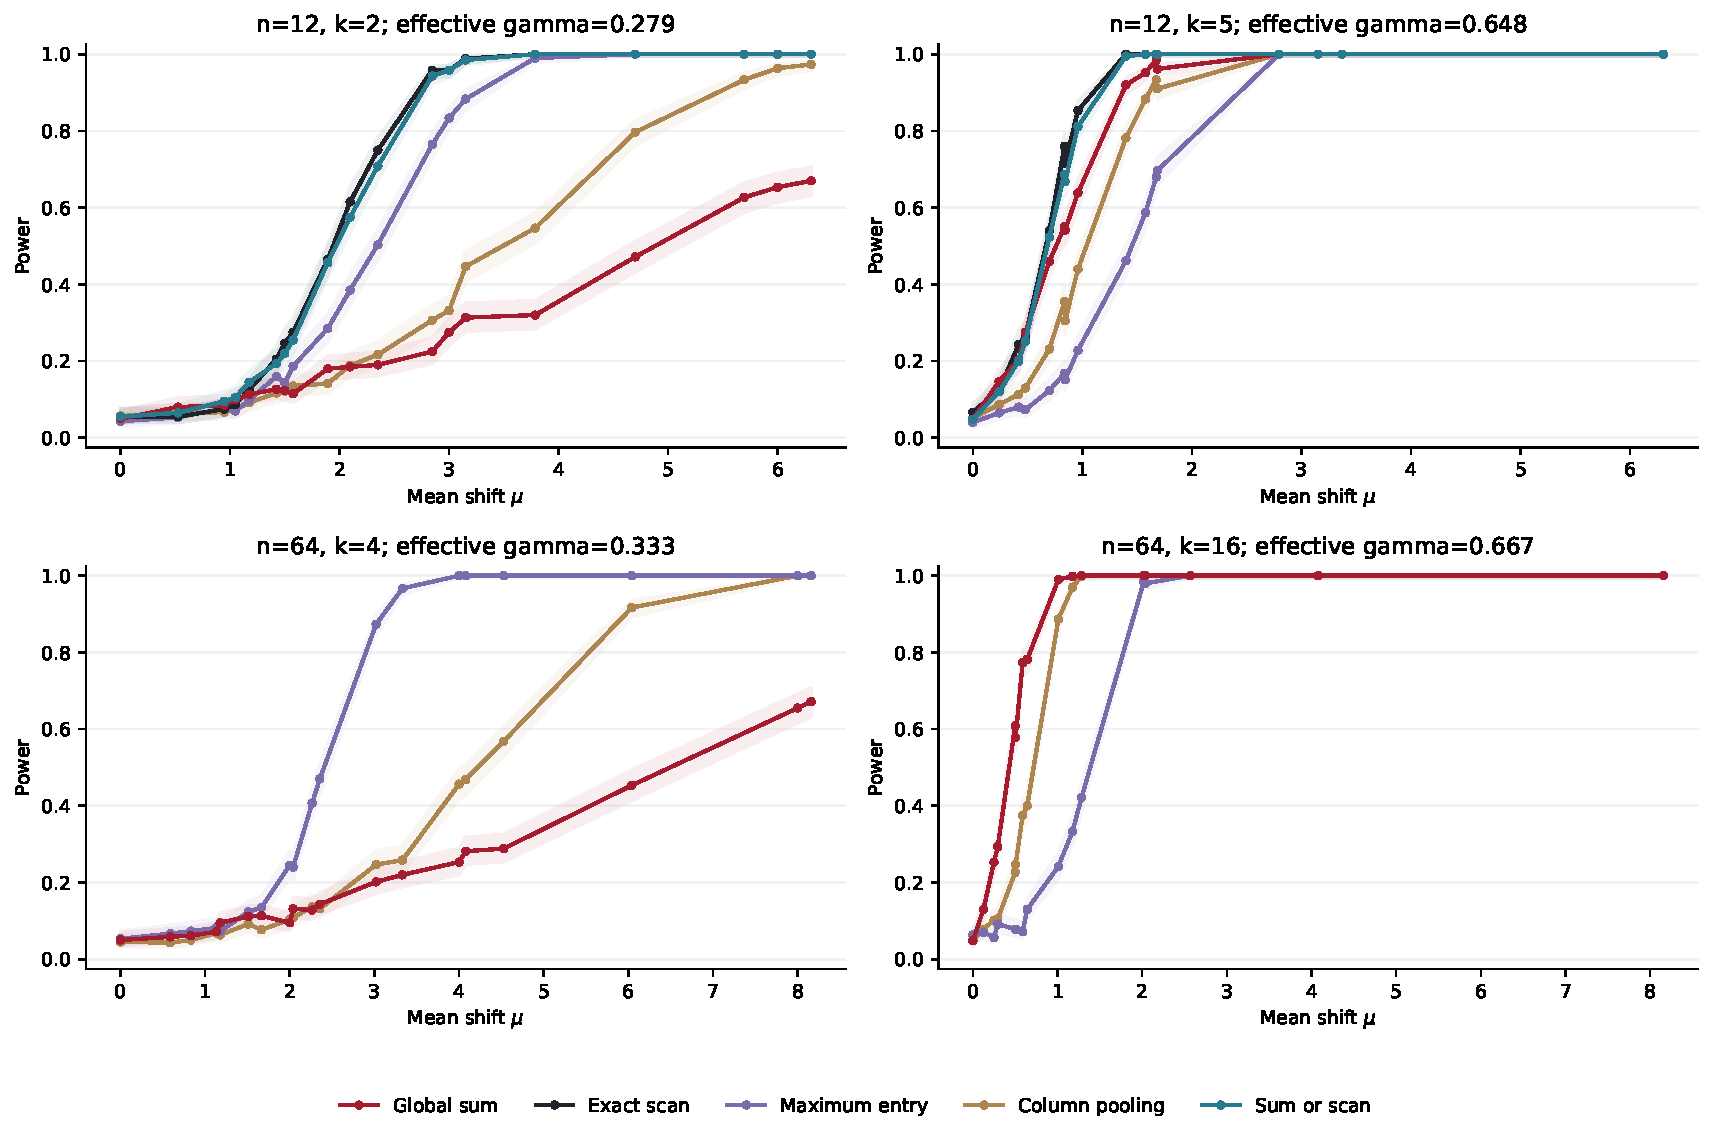
\includegraphics[width=\textwidth]{figures/detection_power.pdf}
\caption{Empirical detection power at nominal level $\alpha=0.05$.
Shaded bands denote marginal Wilson $95\%$ confidence intervals; all
procedures within an experiment are run on paired matrices.}
\label{fig:power-curves}\end{figure}
\begin{figure}[t]\centering
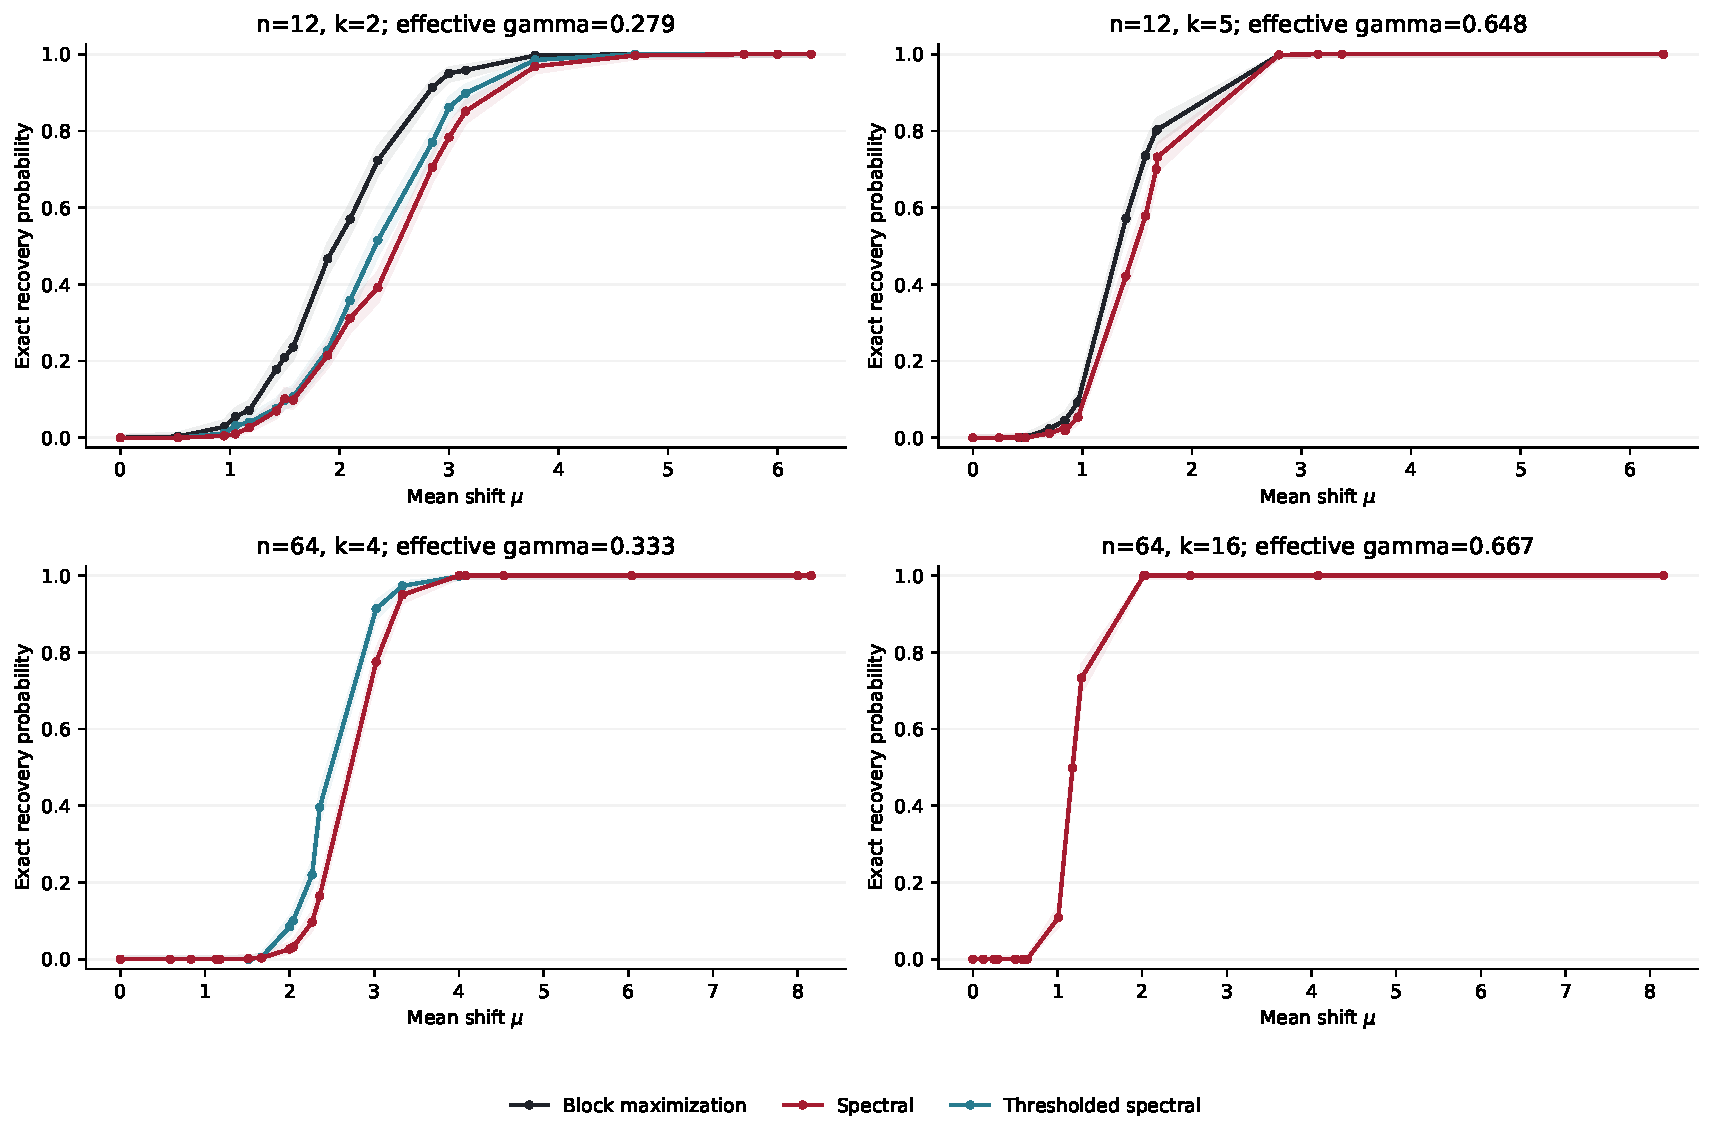
\includegraphics[width=\textwidth]{figures/exact_recovery.pdf}
\caption{Exact recovery probability. An estimate counts as correct only if
both affected row and column index sets match their planted values.}
\label{fig:recovery-curves}\end{figure}

\label{end:main}

\clearpage
\appendix
\section{Detection Calculations}

The sum and scan calculations follow Appendix A.1 of Butucea and
Ingster~\cite{BI2013}. Their large matrix dimensions $N,M$ are both
$n$ here, their submatrix dimensions are both $k$, and their parameter
$a$ is our $\mu$. For Ma and Wu~\cite{MW2015}, the change of notation
is $p=n$ and $\lambda=\mu$.

\subsection{The Sum Test}\label{app:sum}

Since the entries are independent and each has variance one, the
unnormalized sum has variance $n^2$ under both hypotheses. Dividing
by $n$ therefore gives $T_{\mathrm{sum}}$ variance one. Under $H_1$,
exactly $k^2$ entries have mean $\mu$, so the unnormalized sum has
mean $\mu k^2$. Moreover, a linear combination of independent
Gaussian variables is Gaussian. Consequently,
\[
T_{\mathrm{sum}}\sim
\begin{cases}
N(0,1), & H_0\\[2pt]
N(\Delta_n,1), & H_1
\end{cases}
\qquad \Delta_n=\frac{\mu k^2}{n}
\]
Let $c_n$ denote the rejection threshold, so that we reject $H_0$
whenever $T_{\mathrm{sum}}>c_n$. The two errors are
\[
P_0(T_{\mathrm{sum}}>c_n)=\Phi(-c_n)
\qquad
\sup_{S,T}P_{S,T,\mu}(T_{\mathrm{sum}}\leq c_n)
=\Phi(c_n-\Delta_n)
\]
These are the expressions used in the paper's proof. Its upper bound
on the Type II error is an equality in our common-mean model.

Following their threshold choice, suppose $\Delta_n\to\infty$ and
take $c_n\to\infty$ with $c_n\leq\eta\Delta_n$ for a fixed
$0<\eta<1$. Then the Type I error tends to zero and
\[
\sup_{S,T}P_{S,T,\mu}(T_{\mathrm{sum}}\leq c_n)
\leq\Phi\bigl(-(1-\eta)\Delta_n\bigr)\longrightarrow0
\]
Thus, the sum test gives reliable detection when $\mu k^2/n\to\infty$.

\subsection{The Scan Test}\label{app:scan}

For fixed $A,B$ with $|A|=|B|=k$, the unnormalized candidate sum
has variance $k^2$. Hence $Z_{A,B}\sim N(0,1)$ under $H_0$.
Under an alternative, the true candidate satisfies
$Z_{S,T}\sim N(\mu k,1)$.

For any proposed rejection threshold $u>0$, a union bound gives
\[
P_0(T_{\mathrm{scan}}>u)
\leq\sum_{\substack{A,B\subseteq[n]\\|A|=|B|=k}}
P_0(Z_{A,B}>u)
=M_n\Phi(-u)
\]
This does not require independence between candidate sums, which is
important because overlapping submatrices share observations.

Set the rejection threshold to $h_n=\sqrt{2\log M_n}$, so that we
reject when $T_{\mathrm{scan}}>h_n$. Butucea and Ingster use the Gaussian
tail estimate
\[
\Phi(-u)\asymp\frac{e^{-u^2/2}}{u}
\qquad\text{as }u\to\infty
\]
Here, $\asymp$ means that the quantities are bounded above and below
by fixed positive multiples of one another for sufficiently large
$u$. Since $M_n\to\infty$, we have $h_n\to\infty$, and their
argument gives
\[
P_0(T_{\mathrm{scan}}>h_n)
\leq M_n\Phi(-h_n)
=O\left(\frac{M_ne^{-h_n^2/2}}{h_n}\right)
=O\left(\frac1{h_n}\right)\longrightarrow0
\]
The final equality follows from $h_n^2/2=\log M_n$. The factor
$1/h_n$ makes the error vanish at this threshold.

We next control the Type II error. Under any alternative, the maximum
includes the true block, so $T_{\mathrm{scan}}\geq Z_{S,T}$.
Consequently,
\begin{align*}
P_{S,T,\mu}(T_{\mathrm{scan}}\leq h_n)
&\leq P_{S,T,\mu}(Z_{S,T}\leq h_n)\\
&=\Phi(h_n-\mu k)
\end{align*}
The bound is independent of $S,T$, so it also holds for the worst-case
Type II error.

Equation (A.1) of the paper gives, in the square case,
\[
\log M_n\sim2k\log(n/k)
\qquad h_n\sim2\sqrt{k\log(n/k)}
\]
The condition $\liminf\mu^2k/[4\log(n/k)]>1$ therefore gives a fixed
multiplicative separation between $\mu k$ and $h_n$. Since
$h_n\to\infty$, their difference tends to infinity, so the Type II
error also vanishes. This is the square specialization of condition
(2.5) in their Theorem 2.1.

\subsection{The Maximum-Entry Test}\label{app:max}

Lemma 1, equation (12), of Ma and Wu~\cite{MW2015} states that, for
$u_n=\sqrt{(4+\varepsilon)\log n}$ with fixed $\varepsilon>0$,
\[
R_n\!\left(\mathds{1}_{\{T_{\mathrm{max}}>u_n\}}\right)
\leq n^{-\varepsilon/2}
+\exp\left[-\frac12(\mu-u_n)_+^2\right]
\]
Here, $x_+=\max\{x,0\}$. We follow their argument in Section 6.1.
Under $H_0$, a union bound and the Gaussian Chernoff bound used
there give
\[
P_0(T_{\mathrm{max}}>u_n)
\leq n^2\Phi(-u_n)
\leq n^2e^{-u_n^2/2}
=n^{-\varepsilon/2}
\]
Under $H_1$, choose an affected entry $X_{ij}\sim N(\mu,1)$.
Since $T_{\mathrm{max}}\geq X_{ij}$,
\[
P_{S,T,\mu}(T_{\mathrm{max}}\leq u_n)
\leq P_{S,T,\mu}(X_{ij}\leq u_n)
=\Phi(u_n-\mu)
\leq\exp\left[-\frac12(\mu-u_n)_+^2\right]
\]
This holds for every location and gives the stated total error bound.
In Section 4.3, the authors apply it under the second condition in
(17) of Theorem 2. If $\liminf\mu/(2\sqrt{\log n})>1$, taking
$\varepsilon$ sufficiently small makes $\liminf\mu/u_n>1$, and
both error bounds tend to zero.

\clearpage
\begin{thebibliography}{99}

\bibitem{BI2013}
Butucea, C., and Ingster, Y.~I. (2013).
Detection of a sparse submatrix of a high-dimensional
noisy matrix.
\emph{Bernoulli}, \textbf{19}(5B), 2652--2688.
\href{https://doi.org/10.3150/12-BEJ470}{doi.org/10.3150/12-BEJ470}.

\bibitem{MW2015}
Ma, Z., and Wu, Y. (2015).
Computational barriers in minimax submatrix detection.
\emph{The Annals of Statistics},
\textbf{43}(3), 1089--1116.
\href{https://doi.org/10.1214/14-AOS1300}{doi.org/10.1214/14-AOS1300}.

\bibitem{BIS2015}
Butucea, C., Ingster, Y.~I., and Suslina, I.~A. (2015).
Sharp variable selection of a sparse submatrix
in a high-dimensional noisy matrix.
\emph{ESAIM Probab. Stat.},
\textbf{19}, 115--134.
\href{https://doi.org/10.1051/ps/2014017}{doi.org/10.1051/ps/2014017}.

\bibitem{CLR2017}
Cai, T.~T., Liang, T., and Rakhlin, A. (2017).
Computational and statistical boundaries for
submatrix localization in a large noisy matrix.
\emph{The Annals of Statistics},
\textbf{45}(4), 1403--1430.
\href{https://doi.org/10.1214/16-AOS1488}{doi.org/10.1214/16-AOS1488}.


\end{thebibliography}

\end{document}

% Original working log from the supplied draft.
% \section*{Project Tracker}
% 
% \renewcommand{\arraystretch}{1.8}
% \begin{tabularx}{\textwidth}{|l|l|X|}
% \hline
% \textbf{Date} & \textbf{Who} & \textbf{What} \\
% \hline
%  10/25/2026 & Faris & created doc. wrote intro \\
% \hline
%  10/25/2026 & Amrit & fleshed out outline. wrote draft of all of 2. made bibliography \\
% \hline
% 10/30/2026 & Amrit & wrote draft of all of 3 and 4. \\
% \hline
% 11/2/2026  & Faris & Read what you wrote. just some ideas and notes. I think we should focus the project on a couple of different tests and their uses (we dont have to cover everything, would be a bit too much as tracy might suspect ai cuz who can read and understand all these papers) \newline \newline ~~~~~~~~~~~~~~~~~~
% if instead like eg through 2 through 2.2 there is some theory development and rigor as opposed to section 3 which is just stating results. I mean these "other tests" and or other questions should be like a page max with a paragraph of discussion for each because the assumption is that we read these like 2-3 main papers that develop the results we are summarizing in depth. \\
% \hline
% 11/5/2026 & Faris & Changed a lot. added more theory and explanations. removed the sections that just stated results as need to rewrite \\
% \hline
% \end{tabularx}